\chapter[Moteur de Scan \& Orchestration]{Réalisation : Moteur de Scanning \& Orchestration Asynchrone}
\label{chap:scan}

\section{Flux Opérationnel Complet d'un Audit de Bout en Bout}
Avant de détailler chaque composant technique, il est essentiel de comprendre le parcours complet d'un audit depuis le clic de l'auditeur jusqu'à la génération du rapport officiel. La Figure \ref{fig:scan_pipeline} décrit ce flux en huit étapes séquentielles :

\begin{figure}[!htbp]
\centering
\footnotesize
\begin{verbatim}
  UTILISATEUR                      FRONTEND (Next.js 16)
  ┌─────────────────┐     ┌───────────────────────────────────────┐
  │ 1. Saisie URL   │────>│ 2. Contrôle RBAC (viewer => blocage)  │
  │    + Mode Scan   │     │ 3. Normalisation HTTPS + jauge 0-92%  │
  └─────────────────┘     └───────────────┬───────────────────────┘
                                          │ POST /api/scans/run
                                          v
  BACKEND (FastAPI)        ┌───────────────────────────────────────┐
  ┌─────────────────┐     │ 4. Validation Pydantic (ScanRequest)  │
  │ PostgreSQL 16   │<────│ 5. get_or_create_website() +          │
  │   (19 tables)   │     │    create_scan(status="running")      │
  └─────────────────┘     └───────────────┬───────────────────────┘
                                          │
                                          v
  ORCHESTRATEUR            ┌───────────────────────────────────────┐
  (orchestrator.py)        │ 6. asyncio.gather() par phases :      │
                           │    Phase 1: SSL, Headers, Cookies, CSP│
                           │    Phase 2: DNS, Email, .git, Stack   │
                           │    Phase 3: ZAP, Nmap, EASM, CTI     │
                           └───────────────┬───────────────────────┘
                                           │
                                           v
  SCORE ENGINE             ┌───────────────────────────────────────┐
  (score_engine.py)        │ 7. Normalisation Finding + Scoring    │
                           │    pondéré + Grade A+ à F + Étoiles   │
                           └───────────────┬───────────────────────┘
                                           │
                                           v
  CLÔTURE & SOC            ┌───────────────────────────────────────┐
                           │ 8. complete_scan() => PostgreSQL      │
                           │    + WebSocket broadcast              │
                           │    + Notification Jrès (TopBar)       │
                           │    + Audit Trail (non-répudiation)    │
                           │    + Contexte IA Amina (localStorage) │
                           │    + Export PDF 7 pages (SHA-256)     │
                           └───────────────────────────────────────┘
\end{verbatim}
\caption{Pipeline opérationnel complet d'un audit CyberScore TN de bout en bout}
\label{fig:scan_pipeline}
\end{figure}

\subsection{Étape 1 \& 2 : Saisie, Normalisation \& Contrôle RBAC Préalable}
Lorsqu'un utilisateur accède à la page \texttt{/scan}, il saisit l'URL du domaine étatique cible (ex: \texttt{finances.gov.tn}) et sélectionne l'un des trois modes d'audit (Quick, Standard ou Deep). Avant toute requête réseau, le composant \texttt{ScannerClient.tsx} effectue un \textbf{contrôle d'habilitation RBAC} :
\begin{itemize}
    \item \textbf{\texttt{Admin}} et \textbf{\texttt{Auditor}} : Autorisés à déclencher l'audit.
    \item \textbf{\texttt{Viewer}} : \textbf{Bloqué immédiatement} — une modale d'interdiction s'affiche, indiquant que le profil est restreint à la consultation en lecture seule.
\end{itemize}
L'URL saisie est ensuite nettoyée (suppression des espaces, ajout automatique du préfixe \texttt{https://} si absent). L'interface active une jauge de progression animée (de 0\% à 92\%) en attendant la réponse de l'API.

\subsection{Étape 3 : Appel API REST \& Validation Pydantic}
Le navigateur émet une requête HTTP \texttt{POST /api/scans/run} vers le serveur FastAPI avec le corps JSON suivant :
\begin{lstlisting}[language=Python, caption={Schema Pydantic de la requete de scan}]
class ScanRequest(BaseModel):
    url: str          # ex: "https://www.finances.gov.tn"
    scan_type: str    # "quick", "standard" ou "deep"
\end{lstlisting}
Le routeur \texttt{scan\_routes.py} valide la conformité du schéma via Pydantic. Si le \texttt{scan\_type} ne figure pas parmi les trois valeurs autorisées, une erreur HTTP 400 est renvoyée.

\subsection{Étape 4 : Persistance PostgreSQL Avant Exécution}
Avant le lancement des scanners, deux opérations de persistance sont effectuées dans la base PostgreSQL 16 :
\begin{enumerate}
    \item \textbf{\texttt{get\_or\_create\_website(db, url)}} : Vérifie si le domaine existe déjà dans l'inventaire étatique des 120 institutions ; sinon, une nouvelle entrée est créée et rattachée au secteur public correspondant.
    \item \textbf{\texttt{create\_scan(db, website\_id, url, scan\_type)}} : Insère un enregistrement d'audit avec l'état initial \texttt{status = "running"}, génère un \texttt{scan\_id} unique auto-incrémenté et enregistre l'horodatage de démarrage.
\end{enumerate}
Ce mécanisme garantit que chaque tentative d'audit est tracée en base de données, même en cas d'échec ultérieur du scan lui-même.

% ================================================================
\section{Architecture Modulaire des 16 Piliers d'Audit}
Le cœur technique de CyberScore TN réside dans sa capacité à auditer passivement les cibles étatiques sans déclencher de perturbation de service et sans requérir d'agent logiciel sur le serveur distant.

Les seize facteurs de risque analysés sont implémentés au sein de \textbf{huit modules Python spécialisés} totalisant plus de 120 Ko de code de sécurité :

\begin{table}[!htbp]
\centering
\caption{Répartition technique des 16 facteurs de risque par module d'audit}
\label{tab:scanners_modules}
\begin{singlespace}
\footnotesize
\renewcommand{\arraystretch}{1.08}
\begin{tabularx}{\textwidth}{p{2.6cm} l X p{3.6cm}}
\toprule
\textbf{Module Source} & \textbf{Fichier Backend} & \textbf{Piliers Techniques Audités} & \textbf{Bibliothèques \& Outils} \\
\midrule
\textbf{Chiffrement SSL} & \texttt{ssl\_scanner.py} & Protocoles TLS 1.0 à 1.3, Cipher Suites, Autorité TunTrust/ANCE & \texttt{sslyze}, \texttt{cryptography}, \texttt{ssl} \\
\textbf{En-têtes HTTP} & \texttt{headers\_scanner.py} & HSTS (\textit{Preload}), X-Frame-Options, Permissions-Policy & \texttt{httpx} (client asynchrone) \\
\textbf{Santé DNS} & \texttt{dns\_scanner.py} & Signatures DNSSEC, Enregistrements CAA, Redondance NS & \texttt{dnspython} (résolveur async) \\
\textbf{Messagerie} & \texttt{email\_scanner.py} & Anti-spoofing SPF, DKIM, Alignement DMARC (\texttt{p=reject}) & \texttt{dnspython} \\
\textbf{Sécurité Web} & \texttt{web\_scanners.py} & Flags Cookies (\texttt{HttpOnly}, \texttt{Secure}), Fuites \texttt{.git}/\texttt{.env}, Stack & \texttt{httpx}, moteurs de regex \\
\textbf{Analyses CTI} & \texttt{advanced\_scanners.py} & Supply Chain CDN sans SRI, Réputation CTI (AbuseIPDB, VirusTotal) & \texttt{httpx}, APIs CTI, parseur DOM \\
\textbf{Scanners Docker} & \texttt{docker\_scanners.py} & DAST OWASP ZAP, Scan 100 ports Nmap, Sous-domaines Subfinder & Docker Engine API, \texttt{zap2docker} \\
\textbf{Socle Abstrait} & \texttt{base.py} & Modèle standardisé \texttt{Finding} et normalisation trilingue & Pydantic v2, \texttt{asyncio} \\
\bottomrule
\end{tabularx}
\end{singlespace}
\end{table}

% ================================================================
\section{Description Détaillée des Sondes d'Audit}
Chaque scanner est une coroutine Python autonome encapsulée avec un \textbf{timeout individuel strict} (5 à 10 secondes). Si un serveur distant met trop de temps à répondre, la sonde retourne un résultat dégradé sans bloquer les autres scanners. Voici le rôle précis de chaque sonde :

\subsection{Phase 1 : Périmètre Web Immédiat \& Chiffrement (Tous Modes)}
\begin{enumerate}
    \item \textbf{SSLScanner} (\texttt{ssl\_scanner.py}) : Établit un handshake TLS avec le serveur cible, teste les protocoles supportés (rejet de TLS 1.0/1.1 obsolètes, validation de TLS 1.2 et TLS 1.3), vérifie la solidité des suites de chiffrement (\textit{Cipher Suites}), la date de validité du certificat X.509 et sa signature par une autorité reconnue (notamment \textbf{TunTrust / ANCE AS2609}).
    \item \textbf{HeadersScanner} (\texttt{headers\_scanner.py}) : Inspecte la réponse HTTP brute à la recherche des en-têtes de sécurité obligatoires : \texttt{Strict-Transport-Security} (HSTS avec option \texttt{preload}), \texttt{X-Frame-Options} (anti-clickjacking), \texttt{X-Content-Type-Options: nosniff}, \texttt{Referrer-Policy} et \texttt{Permissions-Policy}.
    \item \textbf{CookieScanner} (\texttt{web\_scanners.py}) : Examine les attributs des cookies renvoyés via \texttt{Set-Cookie} : présence impérative des drapeaux \texttt{Secure} (transmission HTTPS exclusive), \texttt{HttpOnly} (inaccessibles en JavaScript pour contrer le vol de session) et \texttt{SameSite=Lax/Strict} (anti-CSRF).
    \item \textbf{CSPScanner} (\texttt{web\_scanners.py}) : Analyse la directive \texttt{Content-Security-Policy} pour vérifier le confinement des scripts, styles et iframes, et sanctionne les règles permissives vulnérables au XSS (\texttt{unsafe-inline}, \texttt{unsafe-eval}).
\end{enumerate}

\subsection{Phase 2 : Infrastructure DNS, Messagerie \& Hygiène (Standard \& Deep)}
\begin{enumerate}
    \setcounter{enumi}{4}
    \item \textbf{DNSScanner} (\texttt{dns\_scanner.py}) : Interroge les serveurs DNS souverains tunisiens, vérifie la chaîne de confiance cryptographique \textbf{DNSSEC} (enregistrements \texttt{DNSKEY}, \texttt{RRSIG}, \texttt{DS}) pour empêcher le détournement de trafic, les enregistrements \texttt{CAA} et la redondance des serveurs \texttt{NS}.
    \item \textbf{EmailSecurityScanner} (\texttt{email\_scanner.py}) : Analyse la configuration anti-usurpation de la messagerie du ministère : conformité \textbf{SPF} (serveurs autorisés à émettre), présence de signatures \textbf{DKIM} et politique stricte \textbf{DMARC} (\texttt{p=reject} ou \texttt{p=quarantine}).
    \item \textbf{InfoDisclosureScanner} (\texttt{web\_scanners.py}) : Teste passivement l'accessibilité de chemins sensibles exposés par négligence : \texttt{/.git/}, \texttt{/.env}, \texttt{phpinfo.php}, fichiers de sauvegarde \texttt{.bak} ou dumps de bases de données.
    \item \textbf{TechDetectionScanner} (\texttt{advanced\_scanners.py}) : Identifie le serveur web (Nginx, Apache, IIS) et le CMS/framework via les signatures HTTP, et pénalise la fuite de versions logicielles précises (\texttt{server\_tokens on}).
    \item \textbf{SupplyChainScanner} (\texttt{advanced\_scanners.py}) : Détecte les scripts JavaScript et polices externes chargés depuis des CDNs tiers et vérifie l'intégrité des sous-ressources (\textbf{SRI} avec hash SHA-384).
    \item \textbf{CertManagementScanner} (\texttt{advanced\_scanners.py}) : Calcule la marge de renouvellement avant expiration du certificat X.509 et détecte les certificats \textit{wildcard} non compartimentés.
\end{enumerate}

\subsection{Phase 3 : Scans Actifs Conteneurisés \& Renseignement Cyber (Deep)}
\begin{enumerate}
    \setcounter{enumi}{10}
    \item \textbf{OWASPScanner} (\texttt{docker\_scanners.py}) : Déclenche une instance Docker OWASP ZAP pour tester les failles d'injection web (SQL Injection, XSS, CSRF).
    \item \textbf{NetworkScanner} (\texttt{docker\_scanners.py}) : Exécute un scan Nmap rapide sur les 100 ports TCP les plus exposés (SSH 22, RDP 3389, MySQL 3306, etc.) pour mesurer la surface d'attaque réseau.
    \item \textbf{SubdomainScanner} (\texttt{docker\_scanners.py}) : Énumère la surface d'attaque externe (EASM) via les registres de transparence de certificats (\texttt{crt.sh}) et le moteur Subfinder.
    \item \textbf{ThreatIntelScanner} (\texttt{advanced\_scanners.py}) : Croise l'adresse IP publique du serveur avec les bases mondiales de réputation CTI (AbuseIPDB, VirusTotal) pour détecter toute compromission ou inscription en liste noire.
    \item \textbf{HistoricalComplianceScanner} (\texttt{advanced\_scanners.py}) : Compare les résultats actuels avec l'historique des audits précédents pour identifier les régressions de sécurité.
\end{enumerate}

% ================================================================
\section{Modèle de Données Standardisé : La Structure \texttt{Finding}}
Pour unifier le traitement des données issues de sources hétérogènes, chaque scanner produit des objets normalisés \texttt{Finding} validés par Pydantic :

\begin{lstlisting}[language=Python, caption={Definition Pydantic du modele Finding unifie}]
class Finding(BaseModel):
    category: str           # ex: "ssl", "headers", "dns", "owasp"
    title: str              # ex: "Absence d'en-tete HSTS strict"
    severity: str           # "critical", "high", "medium", "low", "info"
    description: str        # Analyse contextuelle du risque
    remediation: str        # Prescription technique de durcissement
    owasp_category: str     # ex: "A05:2021 (Security Misconfiguration)"
    nist_function: str      # ex: "PR.DS-2" (Protect - Data Security)
    iso27002_control: str   # ex: "A.8.24" (Cryptographie)
    cvss_score: float       # ex: 7.5
    evidence: dict          # En-tetes recus, reponse brute, port detecte
\end{lstlisting}

\subsection{Triple Mapping Réglementaire}
Chaque vulnérabilité détectée est systématiquement annotée selon trois référentiels de sécurité internationaux, garantissant la conformité multidimensionnelle de l'évaluation :
\begin{itemize}
    \item \textbf{OWASP Top 10 (2021)} : Classification par catégorie de risque applicatif (ex: \texttt{A05:2021 — Security Misconfiguration} pour un en-tête HSTS manquant).
    \item \textbf{NIST Cybersecurity Framework v2.0} : Correspondance avec les fonctions et contrôles du cadre fédéral américain (ex: \texttt{PR.DS-2} — \textit{Protect: Data Security}).
    \item \textbf{ISO/IEC 27002:2022} : Alignement sur les contrôles de la norme internationale de sécurité de l'information (ex: \texttt{A.8.24} — \textit{Cryptographie}).
\end{itemize}
Ce triple mapping permet au rapport d'audit de servir simultanément les besoins techniques des officiers RSSI et les exigences de conformité réglementaire de l'ANCS vis-à-vis du Décret-loi n° 2023-17.

% ================================================================
\section{Calibration des 3 Modes de Scan \& Durées Mesurées}
L'orchestrateur (\texttt{orchestrator.py}) exécute les modules selon trois niveaux de profondeur d'audit adaptés aux besoins opérationnels :

\begin{table}[!htbp]
\centering
\caption{Comparatif des 3 modes d'audit et métriques temporelles réelles}
\label{tab:modes_scan}
\begin{singlespace}
\footnotesize
\renewcommand{\arraystretch}{1.05}
\begin{tabularx}{\textwidth}{p{2.8cm} c X p{4.8cm}}
\toprule
\textbf{Mode d'Audit} & \textbf{Modules / Durée} & \textbf{Périmètre Technique Audité} & \textbf{Usage Opérationnel} \\
\midrule
\textbf{Quick Scan} \newline \textit{(Audit Rapide)} & 4 mods \newline \textbf{$\sim$ 2.8 s} & SSL/TLS, En-têtes HTTP de sécurité, Cookies, Politique CSP stricte. & Contrôle flash pré-déploiement ou validation de correctif. \\
\midrule
\textbf{Standard Scan} \newline \textit{(Audit Régulier)} & 10 mods \newline \textbf{$\sim$ 7.4 s} & Quick + DNSSEC, DMARC/SPF, Fuites \texttt{.git}, Stack logicielle, Supply Chain. & Audit périodique régulier de la posture globale d'un ministère. \\
\midrule
\textbf{Deep Scan} \newline \textit{(Audit Approfondi)} & 16 mods \newline \textbf{$\sim$ 28.6 s} & Standard + DAST ZAP, Scan 100 ports Nmap, EASM Subfinder, CTI AbuseIPDB. & Homologation d'État et audit approfondi de certification ANCS. \\
\bottomrule
\end{tabularx}
\end{singlespace}
\end{table}

\subsection{Gain de Performance de la Parallélisation Asynchrone}
Grâce à l'utilisation de \texttt{asyncio.gather}, les requêtes réseau sont exécutées en parallèle non-bloquant. Alors qu'une exécution synchrone séquentielle nécessitait en moyenne 85 secondes pour inspecter un site gouvernemental complet, CyberScore TN finalise l'audit Standard en seulement \textbf{7.4 secondes}, représentant un \textbf{gain de vélocité de plus de 11x}.

% ================================================================
\section{Clôture, Persistance \& Écosystème SOC Post-Audit}
Une fois l'ensemble des scanners terminés et le score global calculé par le \texttt{score\_engine.py}, une séquence de clôture en cinq étapes se déclenche automatiquement :

\begin{enumerate}
    \item \textbf{Persistance PostgreSQL (\texttt{complete\_scan})} : La fonction \texttt{complete\_scan(db, scan\_id, result)} enregistre en base la note globale sur 100, la ventilation par catégorie, les compteurs de vulnérabilités (critiques, hautes, moyennes, basses) et la durée réelle d'exécution en millisecondes.
    \item \textbf{Diffusion WebSocket Temps Réel} : Un gestionnaire de connexions (\texttt{ConnectionManager}) maintient les clients abonnés via WebSocket. À la clôture du scan, un message \texttt{\{"type": "complete", "total\_score": ..., "grade": ...\}} est diffusé à tous les observateurs connectés, permettant la mise à jour en temps réel des tableaux de bord distants.
    \item \textbf{Notification SOC dans le Jrès TopBar} : La fonction \texttt{dispatchCyberNotification()} émet un événement personnalisé JavaScript qui incrémente le compteur de la cloche de notification dans la barre de navigation supérieure, avec le grade obtenu et le nombre de failles critiques détectées.
    \item \textbf{Inscription dans le Journal d'Audit Live} : La fonction \texttt{recordAuditLog()} inscrit nominativement l'événement dans le flux \texttt{LIVE FEED} du Journal d'Audit — incluant l'identité de l'auditeur, le domaine ciblé, le score obtenu et l'horodatage à la seconde — garantissant la non-répudiation au sens du Décret-loi n° 2023-17.
    \item \textbf{Injection du Contexte pour l'IA Amina} : Le score, le grade et les failles critiques sont sauvegardés dans \texttt{localStorage} sous la clé \texttt{cyberscore\_last\_scan\_context}, permettant à l'assistante IA Amina 3D d'orienter immédiatement la remédiation sans saisie supplémentaire de l'auditeur.
\end{enumerate}

% ================================================================
\section{Restitution Visuelle des Résultats d'Audit}
L'interface d'audit (\texttt{/scan}) restitue une analyse complète du domaine inspecté : note globale synthétique sur 100, grade alphabétique souverain, diagramme radar des piliers techniques et inventaire détaillé des vulnérabilités avec preuves et remédiations. L'auditeur dispose en outre d'un bouton d'export direct vers le générateur de rapports PDF officiels « Chancellerie » (7 pages, empreinte SHA-256, QR Code de validation) décrit au Chapitre \ref{chap:dashboard} (Figure \ref{fig:scanner_view}).

\begin{figure}[!htbp]
\centering
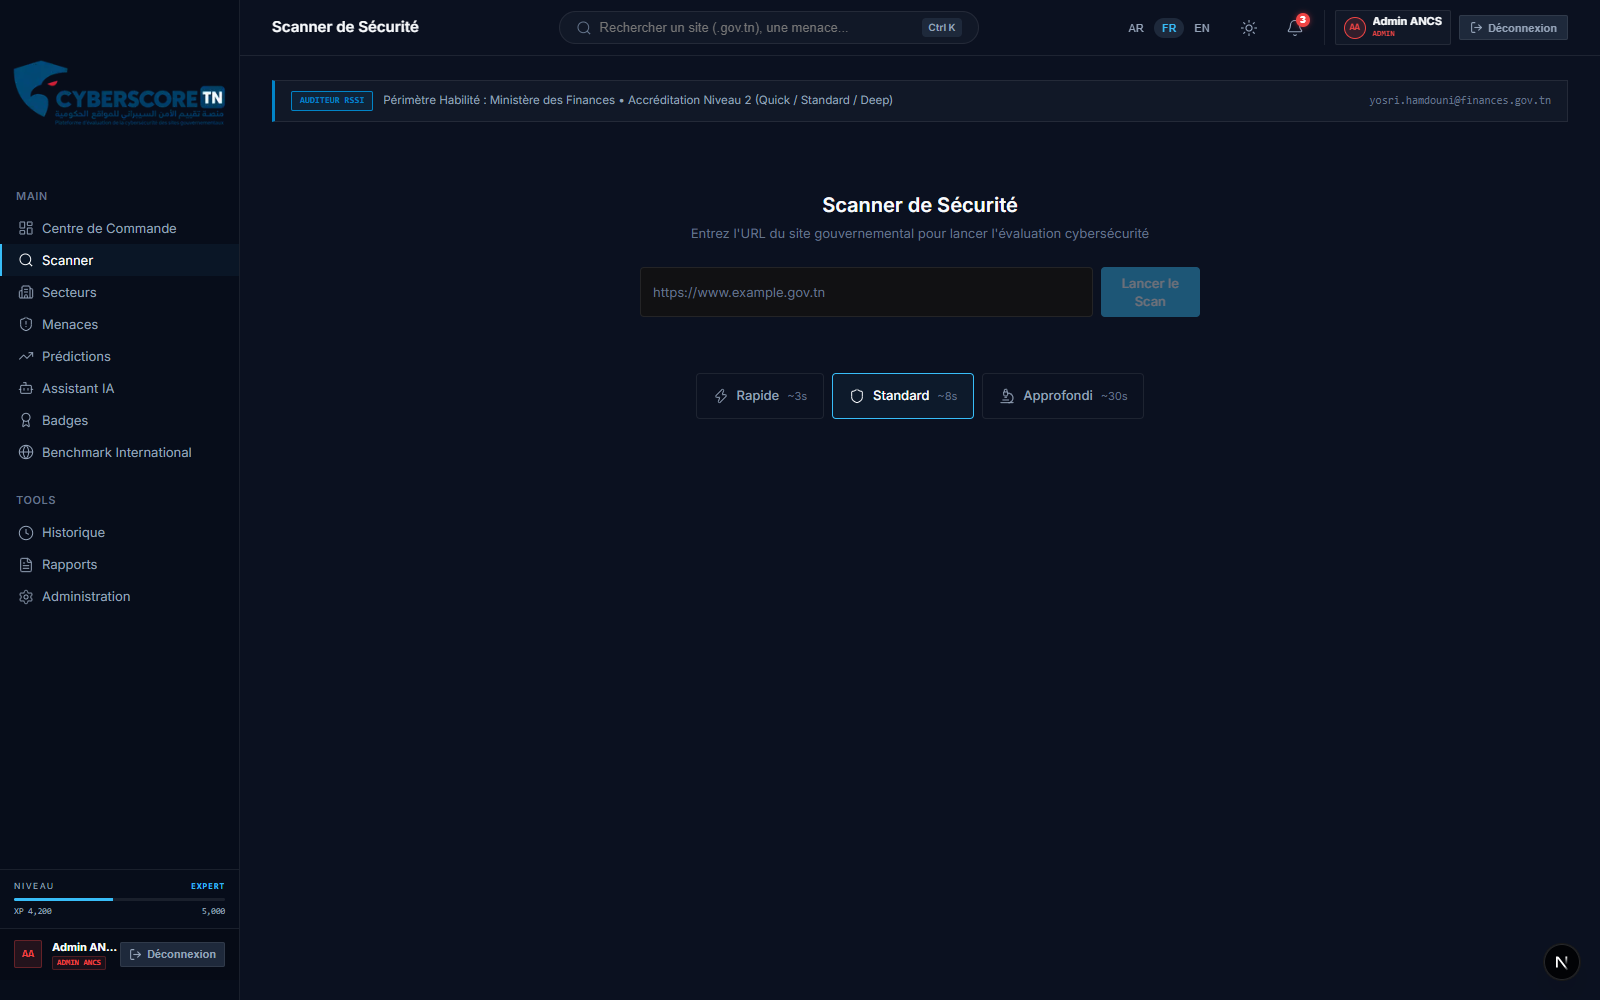
\includegraphics[width=0.70\textwidth]{images/scanner.png}
\caption{Interface d'audit passif et restitution de la fiche technique d'évaluation}
\label{fig:scanner_view}
\end{figure}
